\section{Informacje dodatkowe}

\subsection{napięcia}

Zgodnie z teorią z wykładu: w technologii TTL (Transistor-Transistor Logic)\newline
logiczne zero to napięcie od 0V do 0,8V \newline
logiczne jeden oznacza napięcia od 2,4V do 5V.

\subsection{zbocza}

\begin{figure}[h]
    \centering
    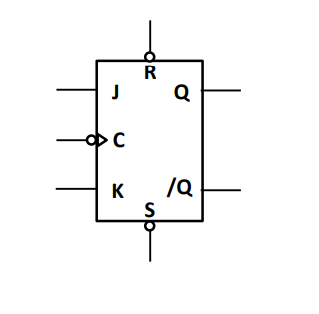
\includegraphics[width=0.4\textwidth]{images/other/jk.png}
    \caption{przerzutnik jk}
    \label{fig:my_label}
\end{figure}

Kółko przy wejściach CLK, RESET, SET oznacza, że dochodzi do zmiany stanu/wyzwolenia na zboczu opadającym czyli podczas przejścia z logicznej jedynki do logicznego zera. Inaczej nazywa się to sterowanie jedynką lub zerem (bez kółek).

\subsection{tabele dla przerzutników}

\begin{table}[h!]
    \centering
    \begin{tabular}{c|c|c||c|c}
        D & Q(t) & Q(t+1) & Q(t) $\rightarrow$ Q(t+1) & D \\
        \hline
        0 & 0 & 0 & 0 $\rightarrow$ 0 & 0 \\
        0 & 1 & 0 & 0 $\rightarrow$ 1 & 1 \\
        1 & 0 & 1 & 1 $\rightarrow$ 0 & 0 \\
        1 & 1 & 1 & 1 $\rightarrow$ 1 & 1 \\
    \end{tabular}
    \caption{tabela prawdy dla przerzutnika typu D (delay/data)}
    \label{tab:my_label}
\end{table}

\begin{table}[h!]
    \centering
    \begin{tabular}{c|c|c||c|c}
        T & Q(t) & Q(t+1) & Q(t) $\rightarrow$ Q(t+1) & T \\
        \hline
        0 & 0 & 0 & 0 $\rightarrow$ 0 & 0 \\
        0 & 1 & 1 & 0 $\rightarrow$ 1 & 1 \\
        1 & 0 & 1 & 1 $\rightarrow$ 0 & 1 \\
        1 & 1 & 0 & 1 $\rightarrow$ 1 & 0 \\
    \end{tabular}
    \caption{tabela prawdy dla przerzutnika typu T (toggle)}
    \label{tab:my_label}
\end{table}

\begin{table}[h!]
    \centering
    \begin{tabular}{c|c|c|c||c|c|c}
        J & K & Q(t) & Q(t+1) & Q(t) $\rightarrow$ Q(t+1) & J & K \\
        \hline
        0 & 0 & 0/1 & 0/1 & 0 $\rightarrow$ 0 & 0 & - \\
        0 & 1 & 0/1 & 0   & 0 $\rightarrow$ 1 & 1 & - \\
        1 & 0 & 0/1 & 1   & 1 $\rightarrow$ 0 & - & 1 \\
        1 & 1 & 0/1 & 1/0 & 1 $\rightarrow$ 1 & - & 0 \\
    \end{tabular}
    \caption{tabela prawdy dla przerzutnika typu JK (Jedynkujące-Kasujące)}
    \label{tab:my_label}
\end{table}

\begin{table}[h!]
    \centering
    \begin{tabular}{c|c|c|c||c|c|c}
        R & S & Q(t) & Q(t+1) & Q(t) $\rightarrow$ Q(t+1) & R & S \\
        \hline
        0 & 0 & 0/1 & 0/1 & 0 $\rightarrow$ 0 & - & 0 \\
        0 & 1 & 0/1 & 1   & 0 $\rightarrow$ 1 & 0 & 1 \\
        1 & 0 & 0/1 & 0   & 1 $\rightarrow$ 0 & 1 & 0 \\
        1 & 1 & zabroniony & zabroniony & 1 $\rightarrow$ 1 & 0 & - \\
    \end{tabular}
    \caption{tabela prawdy dla przerzutnika typu RS (Reset-Set)}
    \label{tab:my_label}
\end{table}

\;\\
\;\\
\textbf{LEGENDA:}\\
0/1 (w następnej komórce 0/1) - 0 przechodzi w 0 przy danym stanie wejść, 1 przechodzi w 1 przy danym stanie wejść,\\
0/1 (w następnej komórce 1/0) - 0 przechodzi w 1 przy danym stanie wejść, 1 przechodzi w 0 przy danym stanie wejść,\\
zabroniony - w przypadku przerzutników RS nie wolno na wejściach podać dwóch jedynek logicznych (zer, jeśli wejścia są zanegowane), przerzutnik się wysypuje.\\
\textbf{Wytłumaczenie:}\\
Przerzutnik typu D: Delay/Data - przerzuca na wyjście wartość wejścia niezależnie od poprzedniego stanu;\\
Przerzutnik typu T: Toggle - gdy aktywowany przełącza przerzutnik w stan przeciwny poprzedniemu;\\
Przerzutnik typu JK: JedynkującoKasujący - wejście J, gdy aktywowane ustawia wyjście przerzutnika w stan 1, wejście K gdy aktywowane ustawia wyjście przerzutnika w stan 0, gdy oba aktywne, zamienia wyjście na przeciwne poprzedniemu;\\
Przerzutnik typu RS: ResetSet - działa analogicznie do JK, z tym, że wprowadzenie jedynek na obu wejściach jest zabionione; Reset gdy aktywny ustawia na 0 wyjście, Set gdy aktywny ustawia na 1 wyjście.\\
\textbf{Słowa zakończenia}\\
Przerzutniki D, T, JK są synchroniczne (potrzebują wejścia zegarowego), ale nie oznacza to, że nie można robić na nich układów asynchronicznych (wejście zegarowe pierwszego przerzutnika podpinamy do zegara, wejście kolejnego do zanegowanego wyjścia poprzedniego przerzutnika).\\
Przerzutnik RS jest asynchroniczny, nie posiada wejścia zegarowego (można je wprowadzić, w programach realizujących układy istnieją RS synchroniczne, wystarczy dołożyć 2 bramki NAND do Seta i Reseta z CLK.

\subsection{bramki na labach}

W pracowniach na UNILOGACH (nie próbujcie googlować, nie znajdziecie i tak) korzystamy głównie z bramek NAND (2,3,4 wejściowe), NOR (2,3,4 wejściowe), NOT, XOR oraz przerzutników typu D, JK oraz szyn rozszerzających, dlatego większość zadań było dostosowywane do tego, żeby móc wykorzystać tylko powyższe bramki. Na zdalnym egzaminie może nie mieć to większego znaczenia, lecz w poleceniu może znaleźć się fraza "układ na bramkach/przerzutnikach typu...", więc warto o tym pamiętać.

\newpage

\subsection{układy kombinacyjne a sekwencyjne}

Układ kombinacyjny to taki, w którym stan wyjścia zależy tylko od stanu wejść, a sekwencyjny posiada pamięć - wyjście zależy od wejść i stanu poprzedniego.\\
Układ sekwencyjny opisuje 2 funkcje:
\begin{itemize}
    \item delta $(\delta) - Q\times X \rightarrow Q'$
    \item lambda $(\lambda) - Q\times X = Y$ 
\end{itemize}

\subsection{minimum bramek, jakie potrzeba}

Do zbudowania każdego układu wystarczą 3 bramki: NOT, NOR, NAND, każda bardziej złożona bramka czy przerzutnik można zbudować z powyższych.

\subsection{wielka piątka układów cyfrowych}
Piątka dla każdego układu cyfrowego:
\begin{itemize}
    \item Q - zbiór stanów układu,
    \item X - zbiór wejść układu,
    \item Y - zbiór wyjść układu,
    \item $\delta$ - funkcja przejść układu,
    \item $\lambda$ - funkcja wyjść układu.
\end{itemize}
Piątka dla automatów skończonych:
\begin{itemize}
    \item Q - zbiór stanów automatu,
    \item $\sum$ - skończony alfabet wejściowy automatu,
    \item $\delta$ - funkcja przejść automatu,
    \item $q_0$ - stan początkowy układu (należący do Q),
    \item F - zbiór stanów końcowych układu (zawierające się w Q).
\end{itemize}

\subsection{te pościgi, te wybuchy}
\indent\indent Hazard występuje w układach, gdy na żadnej z dróg nie ma sprzężenia zwrotnego, każda prowadzi przez układ kombinacyjny\\
\indent Hazard zasadniczy występuje, gdy na jednej z dróg znajduje się układ kombinacyjny, a druga prowadzi przez układ pamięci\\
\indent Wyścig pojawia się, gdy każda z dróg prowadzi przez układ ze sprzężeniem zwrotnym, na każdej z dróg występuje układ pamięci (sygnał "ściga się", żeby zmienić dwa bity co może naruszyć stabilność układu)\\